\documentclass[conference]{IEEEtran}
\IEEEoverridecommandlockouts
% The preceding line is only needed to identify funding in the first footnote. If that is unneeded, please comment it out.
\usepackage{cite}
\usepackage{amsmath,amssymb,amsfonts}
\usepackage{siunitx}
\usepackage{algorithmic}
\usepackage{graphicx}
\usepackage{multirow}
\usepackage{pgfplots}
\usepackage{tikz}
\usepackage{xcolor}
\usepackage[italian,english]{babel}

\usepackage[utf8]{inputenc}

\def\BibTeX{{\rm B\kern-.05em{\sc i\kern-.025em b}\kern-.08em
    T\kern-.1667em\lower.7ex\hbox{E}\kern-.125emX}}

\newcommand{\todobox}[3]{%
    \colorbox{#1}{\textcolor{white}{\sffamily\bfseries\scriptsize #2}}%
    ~\textcolor{blue}{#3} %
    \textcolor{#1}{$\triangleleft$}%
}
\newcommand{\todo}[1]{\todobox{red}{TODO}{#1}}
\pgfplotsset{compat=1.16}

\begin{document}
\selectlanguage{English}
\title{\LARGE{Attacks in Autonomous Vehicles: a Survey}}

\author{
    \IEEEauthorblockN{Gianluca Travasci}
    \IEEEauthorblockA{
        \textit{Department of Mathematics} \\
        \textit{University of Padova} \\
        gianluca.travasci@studenti.unipd.it 
    }
}

\maketitle

\begin{abstract}
    An autonomous vehicle is a vehicle that can operates and perform actions under its own power. Autonomous vehicles basically works by sensing the environment, collecting information and managing communication with other vehicles. This is done with a combination of cameras, sensors, GPS, radar, LiDAR and computers. These technologies, used together, map vehicle’s position and the proximity in order to take always the best decision. Because of their reliance on these sorts of technologies an autonomous vehicle need to be resilient against cyber attacks on them.
    Furthermore, these vehicles, in order to make always the right decision, must be connected to each other and to some road infrastructure. If these communication channels are not safe an adverasry can potentially steal private information and inject malicious data.
    \newline
    This paper presents an overview of recent research on AV safety failures and security attacks, as well as the available safety and security countermeasures.

\end{abstract}
    
\begin{IEEEkeywords}
    Autonomous vehicles, LiDAR, Camera, Sensor, Security, VANET.
\end{IEEEkeywords}

\section{Introduction}
    There are various levels of autonomous vehicles (AV) depending on the degree of autonomy and in this work we focus on the security of the fully automated vehicles.. In this type of AV all aspects of the dynamic driving tasks, under all roadway and environmental conditions that can be managed by a human driver, are performed by the automated system, and this, potentially without driver present in the vehicle. However, automated vehicles can only work properly with accurate, reliable and trustworthy sensors. Figure 1 give us an overview of how an AV work.
    \newline
    Some example of AVs are the Stanford Shelley [1], AnnieWAY [2] and Google Driverless Car [3]. All of those cars use Light Imaging Detection and Ranging (LiDAR) to detect objects and camera for traffic sign recognition. These two sensors act together to influence the mission planning. When LiDAR detects an obstacle on the road, the mission is replanned to avoid that object. Resilience of AV sensors against attacks is a key challenge. Indeed, any attack that degrades sensor data can cause false driving reaction, leading potentially to accidents and fatalities [4]. For example, if camera is attacked, it can misread a speed limit sign, leading to unsafe driving conditions for the vehicle’s passengers. If a LiDAR detects a fake obstacle because of an attack and triggers an emergency brake, it will seriously alter traffic efficiency if it’s done for example in the highway. 
    \newline
    Furthermore, automated vehicles can communicate with each other and share information about the environment. Communication is not limited to communication between cars or to communication between cars and the infrastructure [5]. A cyber attack can be done with control technology tools that are embedded in AVs such as electrical window controls, which are now controlled by engine control units (ECUs) as embedded systems. The ECU is one of the most important parts of a vehicle [6]. An attacker can modify the programming code during design and implementation processing. This attack is done in order to corrupt or degrade hardware performance, or to destroy informations. In [7] was created a virus that could modify the messages delivered by the controller area network (CAN) bus. Upon successful capture of door locking messages, this virus was able to remotely lock a vehicle’s doors. Security issues involving the CAN bus, which connects to all the vehicle’s components, crate risks for drive safety and privacy. A cyber attacker can configure the settings, modify code, and implant viruses and malware [8][6].
    \newline
    The key contribution of this paper are:
    \begin{itemize}
        \item We present a detailed, accurate and updated overview about the state-of-art of AV safety issue and corresponding countermeasures;
        \item We describe almost all the possible attacks that could be done in AV because this type of work hasn't yet been done before in this way. In our knowledge, we are the first considering all of these scenarios, while other survey focus on only a small subset;
        \item We present also all the opened issue for researchers that aim to join this research field.
    \end{itemize}
    
    
    
    \begin{figure*}
        \centering
        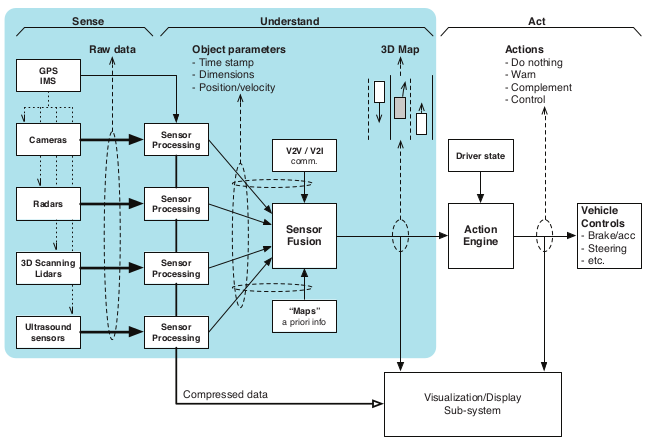
\includegraphics[width=.7\linewidth]{./files/Schermata da 2020-02-13 12-41-35.png}
        \caption{Autonomous vehicle overview.}
        \label{fig:AVoverview}
    \end{figure*}


\section{AV Overview}
\subsection{Security principles}
    Computer security is strictly linked to information security, due  to  its  core  nature:  data. AV, to perform the right decision, has to analyze data taken from sensors, and this make them premium targets of malicious attackers. As a defending mechanism, information security principles should be applied to AV. The three core 
    principles should be achieved:
    \begin{itemize}
        \item confidentiality, for prevent an unauthorized access to data;
        
        \item integrity, for detect an unauthorized access to data and prevent an unauthorized modification to data;
        
        \item availability, for the capability to correctly work all the time.
    \end{itemize}
    Privacy, authenticity, accountability, non-repudiation and reliability are additional properties that AV security might aim to achieve, depending on specific requirements.

\subsection{AV Variety}
    As mentioned before, AV have different level of automation. National Highway Traffic Safety Administration (NHTSA) [9] classifies vehicle automation in six levels:
    
    \begin{itemize}
        \item \textit{No-Automation (Level 0)}At all times, the driver has complete and sole command and control of the vehicle with respect to steering, braking, throttle and motive power;

        \item \textit{Driver Assistance (Level 1)} vehicle is controlled by the driver, but some driving assist features may be included in the vehicle design;
        
        \item \textit{Partial Automation (Level 2)} Vehicle has combined automated functions but the driver must remain engaged with the driving tasks;

        
        \item \textit{Conditional Automation (Level 3)} Driver is necessity, but is not required to monitor the environment. The driver must be ready to take control of the vehicle at all times with notice;

        
        \item \textit{High Automation (Level 4)} The vehicle is capable of performing all driving functions. The driver may have the option to control the vehicle;
        
        \item \textit{Full self-Driving automation (Level 5)} The vehicle is intelligently designed to monitor roadway conditions and act solo, performing all safety–critical driving functions for an entire trip.

    \end{itemize}

\subsection{Challenges and constraints}
    AVs are the future of private and public transports. This is a new research field and a lot of work as to be done especially in the security field. As we will see in the following sections many cyber attacks can be done by using sensors or communication channel leaks. 
    A lot of work as to be done also in the image analysis and computational power instead to perform always the best decision at the right time.

\section{AV security attacks on sensors}

\subsection{Global Positioning System}
    To bypass the difficulties of get GPS data, the count of satellites with public domain is increased so everyone can easily access these data. Because of this an adversary can mislead or manipulate data to provide the wrong directions, to control the routing of the 
    vehicle or to make the vehicle crash [10].
    \newline
    GPS jamming is an attack where the adversary temporarily blocks GPS signals by sending more powerful signal in the same frequency. This type of attack is really effective on AV because to perfectly locate and navigate, autonomous vehicles need to use GPS data with great accuracy [11]. 
    GPS spoofing is an attack where an adversary forges counterfeit GPS signals and send them to the target as valid ones. 
    \newline    
    GPS spoofing relies on GPS jamming to block valid signals before sending the counterfeited ones. GPS spoofing is really effective on AVs for the same reasons  as  GPS  jamming.  Public  GPS  is  not  designed  to  be secure because of its public nature. The only countermeasure to GPS spoofing is authentication, achievable through proper encryption [12].
    \newline    
    Given the fact that GPS are programmed to receive the stronger signals, the adversary  just by sending a strong unrealistic signal can gradually modify the position of the vehicle from the desired target [13]. 
    \newline    
    To prevent this type of attacks researchers developed many simple validation mechanisms that can be put in place. For example monitoring identification codes, satellite signals, and the use of time intervals can help detect spoofing and jamming attempts. 
    \newline    
    In [14]  is detailed how the observed signal strength would be expected to be around 163 decibel watts so a solution could be to block signal with higher frequencies. However, if the attack is sufficient smart enough to appear genuine, these validation checks will fail and the GPS device will be manipulated. 
    \newline
    Q. Yang et al. in [15] combined antijamming and antispoofing algorithm for a GPS receiver based on an antenna array. In their method, the jamming is eliminated by subspace projection, and then a compressed sensing framework is adopted to obtain the direction of arrival (DOA) of the despreading satellite navigation signal and detect the spoofing signal. According to the DOA of the authentic and spoofing signals, the receiver uses adaptive multibeamforming to concurrently achieve the undistorted reception of the authentic satellite signal and the suppression of the spoofing.
    \newline
    However, in our knowledge, a good and realistic solution to prevent these attacks has not yet been found. The only way to avoid GPS Jamming and GPS Spoofing is to implement a military-grade cryptographic.
    
\subsection{Light Detection and Ranging (LiDAR)}
    LiDAR is a type of range-finding sensor that emits light pulses and measures the time it takes to reflect off a distant surface, called a ping. These laser pulses are commonly bounced off of a spinning mirror thousands of times per second, creating a scan of laser pulses. When the original pulse is received more than once, these additional pulses received are called echoes. Echoes are useful to detect objects under almost any weather condition [16].
    \newline
    Relaying signal attack could be seen as an extension of the replay attack where aims is to relay the original signal sent from the target vehicle LiDAR from another position to create fake echos, and eventually move objects from their real position [17]. J. Petit et al. demonstrate that using only two transceivers at the modest cost of 45\$ is possible to perform this attack. Basically the first transceiver is a photodetector sensitive to the LiDAR wavelength (905nm) that produce in output a voltage signal that corresponds to the intensity of the pulse sent by the LiDAR. That output is then sent to the second transceiver, which uses a laser to emit a pulse in return.
    \newline
    Spoofing signal attack is an extension of the previous one and with this one an adversary, by sending a signal of the same frequency to the scanner, can create fake objects. LiDAR typically listen for incoming reflection for at least \SI{1.33}{\micro\second}. To successfully inject signals into the LiDAR, the counterfeit signal should arrive within this window. The earlier the LiDAR receives the signal, the closer it will be to the LiDAR.
    Therefore, if the attacker delays the original signal before it relays it, it can control the position of the objects.
    \newline
    These attacks makes an AV to move slowly or stop and doing this in a highway could also result in the cost of lives [17-20].
    \newline
    \begin{figure}
        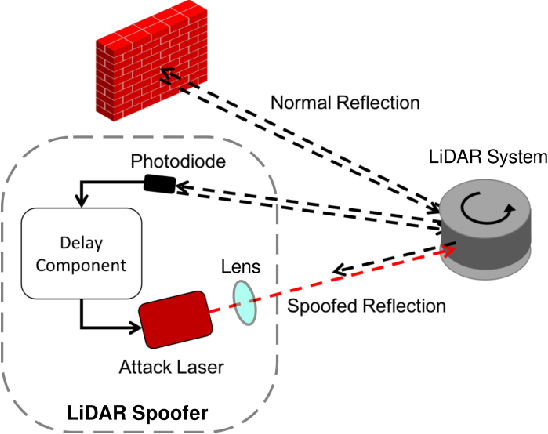
\includegraphics[width=9cm]{./files/lidarspoof.png}
        \caption{Relaying and Spoofing signal attacks on LiDAR.}
    \end{figure}
    Because the attacker need to be synchronized with the pulse interval of LiDAR few possible countermeasures could be:
    \begin{itemize}
        \item non-predictability skip of certain pulses, in this scenario LiDAR skip a pulse but it still listen for incoming pulses. If it notice a response this may indicate that an attacks is going on;
        \item shortening the pulse period of LiDAR we drastically reduce the attack window on the sensor but decreasing the ping period means decrease the working range of the sensor [17].
    \end{itemize}
    What i can understand form these attacks is that LiDAR pulses are not encoded. In our knowledge would be interesting to try adding an encoding of lidar pulses to prevent these attacks.
    
\subsection{Camera}
    A camera is an optical device that can perceive the world as a digital video signal. Cameras are frequently found in AVs for many applications; they are used for lane detection [21], traffic sign recognition [22], headlight detection [23], etc. 
    \newline
    A really effective attack on this sensor is to blind it fully or partially, by emitting light. Failing to detect objects such as speed limit signage or traffic light can put passengers is serious trouble [17]. According to an MIT Technology Review, the Google Driverless Car is susceptible to this problem where low sunlight is able to blind the vehicle’s cameras [24].
    \newline
    Another attack, similar to the previous one, presented in [17] consists on influencing the auto controls in the period before the image recovers and stabilizes after high exposure to a light source. The longer it takes to stabilize to the new environmental conditions, the longer the car is vulnerable to objects it cannot detect. This attack is limited to front/rear/side attack, because it assumes that the attacker continuously switches the light on and off. 
    \newline
    Possible countermeasures are to introduce multiple cameras that provide the same image so the attacker has to put more effort into the attack to blind all cameras at the same time. Integrating a removable near-infrared-cut filter, a technique that is available on security cameras, can filter near-infrared light on request. Another option is to use photochromic lenses. These types of lenses can change color to filter out specific types of light [17]. 

\subsection{Inertial Measurement Units (IMU)}
    IMU is the combination of the Gyroscope and Accelerometers which provides the data of velocity, acceleration, and orientation of the vehicle. They also monitor the change in the environmental dynamics like the gradient. The data provided by the sensors can be modified to not recognize the gradient of the road. 
    \newline
    Karl Koscher et al. in [25] developed CarShark tool to observe data traffic on CAN bus system, performs a detailed packet analysis and modification of packets - simulating a man-in-the-middle attack on the CAN network - and observing the effect on the vehicle. As result they were able to modify sensor’s value through changing data packet.
    \newline
    A possible mitigation system could be to use an encrypted communication on the vehicle’s communication network. Another one could be the use of additional sensors to provide a secondary source of measurement like the GPS. For example, data taken from GPS can help to determine if the vehicle is located on steep gradient.

\section{Vehicular adhoc network (VANET) attacks}
    AVs adopt two main communication mechanisms in order to communicate with the driver, other cars and the road. These are vehicle-to-vehicle (V2V) and vehicle-to-infrastructure (V2I). Figure \ref{fig:Vanet} give us an overview about VANET.
    \newline
    \begin{figure}
        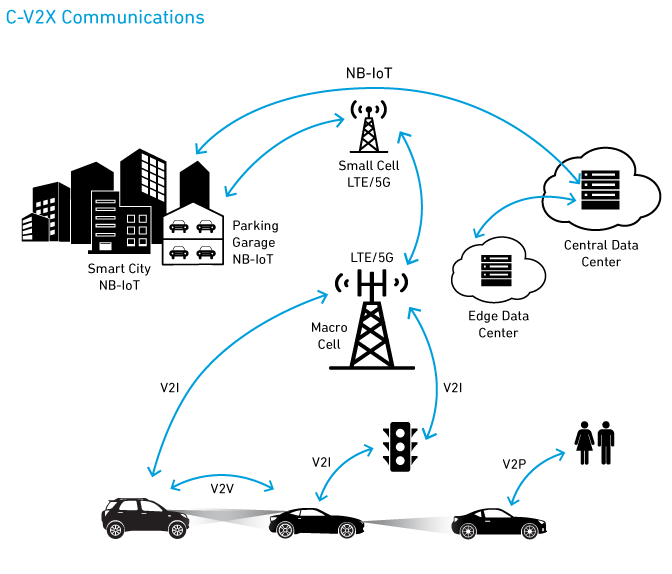
\includegraphics[width=9cm]{./files/fig2_cv2x-communications_720px.png}
        \caption{VANET network.}
        \label{fig:Vanet}
    \end{figure}
    \newline
    V2V communication provide the possibility for vehicles to communicate with each other in a peer-to-peer mechanism. This system uses the IEEE 802.11p protocol where the principle is that when two or more vehicles are in radio communication range, they can connect automatically and establish an ad hoc network where all connected nodes can share information such as position, speed, direction, etc.
    \newline
    V2I communication provide the possibility to connect vehicles to electronic devices in order to control and monitor the physical environment where they are travelling. The informations exchanged between vehicle and infrastructure can be used to optimise the traffic control, to maximise the traffic flow, minimise the fuel usage and control the pollution.

    \subsection{Authenticity/identification attacks}
    Any flaws in the process of authentication/identification may cause serious consequences to the entire network. Cryptographic scheme allows the receivers to verify the origin of the exchanged data. Some examples of authenticity attacks and their corresponding countermeasures are as follows:
    \begin{itemize}
        \item \textit{Sybil attack} is an attack where a malicious vehicle transmits the various messages with multiple fake or stolen source identities to other nodes in the network with a spoofing attack. Therefore legitimate/authenticated nodes consider the malicious messages to be legitimate and cannot detect the real identities of the attackers [26].
        \newline
        Chen et al. [27] proposed a ‘Robust Sybil Attack Detection’ approach based on motion trajectories differences of vehicles. The author has assumed that people driving vehicles on their individual path, chosen speed, and maintains some distance from other vehicular nodes for traffic or passenger safety. Therefore, each vehicle can detect attacks independently with little support from infrastructure. In this approach, infrastructures are made available vehicle’s digital signatures along with timestamp periodically or on-demand. Each motor vehicle is able to independently record these signatures and utilize them during the measure and compare the differences from neighboring node’s signature vectors to detect Sybil nodes.
        \newline
        Another countermeasure for this type of attack is the one proposed by Park et al. in [28]. Basically, in this approach when a vehicle passes through an intelligent traffic infrastructure it acquires certified timestamp that is signed by the infrastructure. A motor vehicle sent a traffic message, which contains a timestamp series to confirm thatwhen a vehicle passes through the last few infrastructures. It is unusual to have two vehicles passing through multiple infrastructures at the similar time, because each vehicles moves with different dynamics. Based on this fact, when a receiver vehicle receives numerous messages with same timestamp series can be detected as Sybil Attack.
        \newline
        This type of attack is well known by the research community and a lot of countermeasures has been developed, [29], [30], [31], we can consider it largely mitigated. 
        
        \item \textit{Replication attack} means one or more nodes claiming an legitimate identity with duplicate keys/certificates.
        J.L. Huang et al. in [32] presented an anonymous batch authenticated and key agreement (ABAKA) scheme to authenticate multiple requests sent from different vehicles and establish different session keys for different vehicles at the same time. ABAKA can efficiently authenticate multiple requests by one verification operation and negotiate a session key with each vehicle by one broadcast message. Elliptic curve cryptography is adopted to reduce the verification delay and transmission overhead. The security of ABAKA is based on the elliptic curve discrete logarithm problem, which is an unsolved NP-complete problem.
        \newline
        Y. Hao et al. in [33] proposed a new cooperative message authentication protocol (CMAP) with an assumption that each safety message carries the location information of the sender vehicle (which can be generated by a global positioning system (GPS) device). Verifiers of each message are defined according to their locations in relation to the sender. Only the selected verifiers check the validity of the message while other vehicles rely on verification results from these verifiers. In the test phase of the protocol it result to be the most effetive one for counter the replication attack.
        \newline 
        Also in this case  we can consider this attack fully mitigated. 
    \end{itemize}
    
    \subsection{Availability attacks}
    The requirement of availability is mandatory to ensure the safety of the involved drivers and vehicles. Due to the major impact on the network resources, DoS attacks are commonly recognized as the most serious threat to the availability of vehicle related systems. Authentication, detection and cryptographic solutions are usually employed to counter such attacks.
    \begin{itemize}
        \item \textit{Malware attack} is to jeopardize the network or software components of the system via any form of hostile or intrusive software like computer viruses. Such attack can be mitigated by using anti-malware software and firewall.
        
        \item \textit{Denial of Service (DOS) attack} has the major purpose to prevent legitimate entities from accessing the network services and resources. Basically, denial-of-service attack means that an adversary floods the  target  with  requests, overloading its resources to disrupt availability.It can also be known as DDOS (Distributed Denial of Service), when multiple computers and/or Internet connections are used to launch the attack. Researchers have demonstrated how DDoS attacks can be performed against VANETs [34] and that it is possible to identify malicious connections for prevention [35], [36], [37]. Different types of DoS attacks can be performed by overwhelming a single network node, V2V or V2I.
        \newline
        He et al. propose a pre-authentication scheme, which taking advantage of the one way hash chain and a group re-keying method to mitigate DoS attack in [38]. 
        \newline
        Verma et al. designs a data structure to filter packets and detect abrupt change, thereby avoiding DoS attack in [39].
        \newline
        This type of attack is well known by the research community and a lot of countermeasures has been developed so we can consider it fully mitigated. 
        
        \item \textit{Wormhole attack} means that the packets captured at one region of the network are transmitted to another region of the network. This would confuse the routing mechanisms where the accuracy of the distance between entities inside the network is crucial [39]. 
        \newline 
        S.M. Safi et al. in [40] propose a way to restrict the packet’s maximum allowed transmission distance, which would ensure that the recipient of the packet is within reasonable range of the sender. This method, called HEAP, is very suitable for VANETs because it has a better performance compared to other authentication methods. HEAP is applicable for all unicast, multicast, and broadcast applications. We can also use HEAP as authenticator for all types of packets.
    \end{itemize}
    
    \subsection{Data integrity attacks}
    Data integrity refers to the fact that the data must be intact and unchanged throughout its lifecycle. The attackers especially those having authenticated entities could easily alter the data or create false data. Thus, secure communication and information encryption are necessary to prevent/mitigate the attacks on data integrity.
    \begin{itemize}
        \item \textit{Masquerading attack} means any attack that uses a forged identity to gain unofficial access to the system. For example, a malicious node disguises itself as an emergency vehicle, and so the surrounding vehicles are tricked into slowing down, changing lane, etc. in order to give way to it.
        \newline 
        T.W. Chima et al. in [41]  proposes a scheme, called SPECS (Secure and Privacy Enhancing Communications Schemes), to ensure the security and privacy issues of V2V communications and detect the masquerading attacks. This approach is based on the idea of IBV (Identity-Based Batch Verification) Scheme [42], which suffers from impersonation attack and cannot fulfill privacy requirements. To protect the identity of each vehicle it uses pseudo-identity and a shared secret key \textit{m} between a vehicle and RSU (Road-Side Unit).
        \newline
        To authenticate a vehicle with a nearby RSU, the scheme uses Public Key Infrastructure (PKI) and assumes that there is a trusted authority (TA) constantly online. A secure fixed network is dedicated for communications between RSUs and TA. To avoid bottleneck, redundant TAs with identical functionalities and databases are installed. It is worth noting that TA is the only authorized component knowing the real identity of vehicles. The vehicle authentication with the TA is performed via RSU. Then TA passes verification information to RSU. RSU then generates a shared secret key mi with the vehicle. If this is the first time that the vehicle authenticates itself with the TA, TA will also pass its master key \textit{s} and a shared secret \textit{m} to the vehicle, via RSU of course. This only needs to be done once in the whole journey. For security reasons, \textit{s} is not preloaded into any vehicle’s hardware. Each time the vehicle passes a new RSU, a new shared-secret key is generated. To generate the signature, vehicle uses the shared secret key and hash function with the signing key. As \textit{m} is only known by the vehicle, RSU and TA, attackers or other vehicles cannot generate the valid signing key to sign the message. RSU always verify the vehicle’s signature even if the vehicle uses pseudo identity to sign the message. Invalid signatures can be detected using a batch verification process by RSU. In IBV (Identity-Based Batch Verification), if any invalid signature is found using the batch verification process the whole batch is dropped.
        \newline
        If an attacker is found, it notifies other vehicles and repeats the process until the search reaches a predefined level or all signatures are validated. After verifying the signature, the RSU broadcasts the message to all vehicles without the hash value, which is stored into positive and negative bloom filters. Any vehicle that wants to know the validity of a received message will create the hash value and compare with the bloom filters hash value. A message is valid if the hash value of this message is found in the positive bloom filter. Otherwise, the message is considered as invalid.
        
        \item \textit{Replay attack}, also known as \textit{Playback attack}, is an attack where data are fraudulently repeated or delayed. State-of-the-art security architectures employing a strong cryptographic system have the potential to effectively thwart application layer attacks in the case where the adversary is an untrusted outsider. Digital signatures provide data integrity for beacon messages and protect them from unauthorized change. Moreover, using nonce in the messages, which is an arbitrary number (chosen in a pseudo-random process) used only once in communication, is a technique to prevent replay attacks [43].
        \newline
        But if we consider the scenario where the adversary is a trusted insider such as a compromised vehicle with a valid certificate, the problem is much harder to solve. Typical approaches to handling this issue are via misbehavior/anomaly detection techniques such as [44], which require multiple sources of data that may not always be available. In addition, such techniques do not guarantee perfect detection in all circumstances, and are usually associated with finite false negative and false positive rates. There is much left to be done in the anomaly detection field to ensure acceptable performance of these algorithms to ensure the safety of passengers.
    \end{itemize}
    
    \subsection{Confidentiality attacks}
    The attacks on confidentiality may not affect safety as previous mentioned attacks do. Nevertheless, the sensitive information exchanged in network, e.g., AVs location, ITS safety messages and driver's personal information, should be protected. Information encryption and secure communication can be used to avoid information leak.
    \begin{itemize}
        \item \textit{Eavesdropping attack:} vehicles periodically broadcast beacons that contain various types of information such as vehicle identity, current vehicle position, speed and acceleration. The availability of this information can comprise the privacy. The adversary can carry out an eavesdropping attack, to extract valuable information about the vehicle stream such as its trace by linking position data, and use it for her own benefit. 
        \newline
        Eavesdropping is a type of passive attack, and hence is difficult to detect, especially in broadcast wireless communication. However, it is possible to prevent the success of eavesdropping by using encryption to achieve data privacy or using anonymity techniques to achieve identity and location privacy. Anonymity is typically implemented using group signatures [45] or short-term certificates (pseudonyms) [46].
    \end{itemize}
    
    \subsection{Vehicle-to-pedestrian (V2P) network}
    The use of smartphones in a road context by drivers and Vulnerable Road Users is rapidly increasing. To reduce the risks related to the influence of smartphone usage in a situation where traffic needs to be considered, a collision prediction algorithm is proposed based on Pedestrian to Vehicle (P2V) and Vehicle to Pedestrian (V2P) communication technologies. A. Hussein et al. in [47] develped this algorithm that using GPS and magnetometer form a pedestrian smartphone and GPS and other sensor on AV can predict the collision angle. 
    \newline
    Figure \ref{fig:Collision} give us an overview of how the algorithm work.
    \begin{figure}
        \centering
        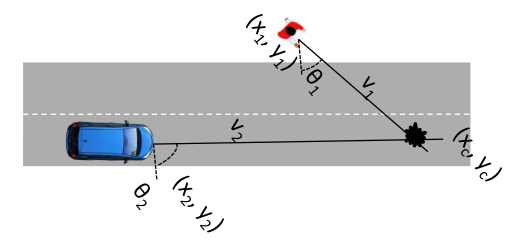
\includegraphics[width=9cm]{./files/Schermata da 2020-02-18 10-20-30.png}
        \caption{Collision prediction angle.}
        \label{fig:Collision}
    \end{figure}
    \newline
    When a collision is calculated a warning message is sent to the pedestrian and to the AV in order to replan the mission and avoid the accident. 
    \newline
    V2P communication is a new research field and not enough work has been done to make this communication safty and resilient. The future is a world where all devices are connected and now a days there are many security issue that makes the "internet of things" not safe enough. 
\section{Hardware attacks}

    \subsection{On-board Diagnostic port (ODB)}
    OBD port is used for collecting diagnostics data of the vehicle. It gives the data about the vehicle faults and performance. It interacts with the ECU communicating through CAN bus. It is a hand held device like USB which has to be connected to the vehicle through the port generally present below the dashboard opposite to adjacent driver seat which then connects to the computer through a wired connection using USB port or through a wireless connection using Bluetooth. 
    \newline
    Y. Zhang et al. in [48] demonstrate that is possible to penetrate several types of cars using OBD port and with this leak they were able to control those cars remotely. 
    Once the on-board PC or device is connected can send and receive data to and from the vehicle ECU’s. W. Yan in [49] shows that in this type of communication is possible an exploitation where data packets can be manipulated for inject malicious packets in to the vehicle networks. Also criminal organizations aim to retrieve information about the intellectual property of Original Equipment Manufacturer and suppliers for creating counterfeit components or about driver sensitive data such as driving behavior.
    \newline
    G. Bose et al. in [50] proposed, as countermeasure, the combination of the seed key protocol with a Two-Way Authentication Method and a Timer Method in order to make the seed and key values difficult to crack.
    Another possible solution to prevent this type of attacks is proposed by D.K. Oka et al. in [51] where they demonstrate the potential of using cryptographic techniques for message authentication of the CAN network to mitigate the transfer of unauthorised data. 
    \newline
    However a concrete solution has yet to be offered. This area of research is largely unaddressed.
    
    \subsection{Engine Control Unit (ECU)}
    CU takes care of the control functionality of the vehicle through the acquisition, the processing and control of the electronic signals.
    C. Vallance in [52] has demonstrated that is possible to compromise ECUs that control core braking functionality by exploiting the onboard Digital Audio Broadcasting radio and injecting packets onto the CAN network. 
    \newline
    S. Checkoway et al. in [53] have  demonstrated how in some cases there are no security provisions from stopping an attacker uploading new firmware. Because by changing ECU firmware is possible to completely reprogram the vehicle’s behaviour it result a potential threat to public safety. However, in the same paper, they show that  the use of asymmetric cryptographic (public-private key) architecture to ensure that the firmware came from a genuine source can mitigate this vulnerability.

\begin{table*}[t]
  \centering
  \begin{tabular}{*{5}{c}}
    \hline 
    Attack type & Attack & Countermeasures & Reference & Classification \\
    \hline
    
    %AUTHENTICITY ATTACKS
    
    Data authenticity & GPS Spoofing & Signal strength monitoring & B. O’Hanlon et al. & Partially mitigated\\
    
    &  & Military-grade cryptography & B. O’Hanlon et al. & \\
    
    & & Anti-spoofing methods & Q. Yang et al. & \\
    
    & Man-In-The-Middle in CAN bus & Cryptography on CAN & K. Koscher et al. & Uncovered \\
    
    & & Secondary misurament source & & \\
    
    & Sybil attack & Motion trajectories differences & Chen et al. & Fully mitigated\\
    
    & & Authentication via certificate & Park et al. & \\
    
    & & Hashing cryptography & Zhou et al. & \\
    
    & & Authentication & Triki et al. & \\
    
    & & Secret information exchange + hardware support & Grover et al. & \\
    
    & Replication attack & Authentication + key agreement & Huang et al. & Fully mitigated\\
    
    &  & Message authentication & Hao et al. & \\
    
    \hline
    %AVAILABILITY ATTACKS
    
    Data availability & GPS Jamming & Military-grade cryptography & B. O’Hanlon et al. & Partially mitigate\\
    
    & & Anti-Jamming methods & Q. Yang et al. & \\
    
    & LiDAR jamming & Filtering data/using other source of data & Petit et al. & Fully mitigated\\
    
    & Camera blind & Multiple camera & Petit et al. & Fully mitigated \\
    & & filter near-infrared & Petit et al. &  \\

    & & photochromic lenses & Petit et al. &  \\
    
    & Malware attack & Anti-malware/Firewall & & Partially mitigated\\
    
    & DoS/DDoS attack & Authentication & He et al. & Fully mitigated\\
    
    & & Filtering & Verma et al. & \\
    
    & Wormhole attack & Authentication & Safi et al. & Fully mitigated \\
    
    \hline
    %DATA INTEGRITY
    
    Data integrity & Replay attack on LiDAR & Filtering data/using other source of data & Petit et al. & Fully mitigated\\
    
    & LiDAR confusion & Filtering data/using other source of data & Petit et al. & \\
    
    & Confusing auto control & Multiple camera & Petit et al. & Fully mitigated \\
    
    & & filter near-infrared & Petit et al. & \\
    
    & & photochromic lenses & Petit et al. & \\
    
    & ODB port tampering &  & Y. Zhang et al. & Uncovered\\
    
    & Exploitation and injection in CAN bus & & W. Yan & Uncovered\\
    
    & & Seed-Key + 2-way Authentication + timer method & G. Bose et al. & Uncovered\\
    
    & & cryptographic in message authentication & D.K. Nilsson et al. & Uncovered\\
    
    & Masquerading attack & Authentication + Detection of malicious component & Chima et al. & \\
    
    & Replay attack (Outsider adversary) & Cryptographic solution & Amoozadeh et al. & Fully mitigated\\
    
    & Replay attack (Insider adversary) & Anomaly detection & Kim et al. & Uncovered \\
    
    \hline
    %DATA CONFIDENTIALITY
    
    Data confidentiality & Eavesdropping & Cryptographic solution (group signatures) & Lin et al. & Partially mitigated \\
    
    & & Cryptographic solution (short-term certificates) & Papadimitratos et al. & Partially mitigated \\
    
    \hline
  \end{tabular}
  \caption{Possible attacks on AVs.}
\end{table*}
\section{Adversarial machine learning (ML) on deep neural networks (DNN)}
    Adversarial ML attacks on DNNs were first observed by Szegedy et al. [54] where they demonstrated that DNNs can be fooled by minimally perturbing their input images at test time, the proposed attack was a gradient-based attack where minimum distance based adversarial examples were crafted to fool the image classifiers. 
    \newline
    Another gradient-based attack was proposed by Goodfellow et al. [55]. In this attack, they formulated adversarial ML as a min-max problem and adversarial examples were produced by calculating the lower bound on the adversarial perturbations. This method was termed as FGSM and is still considered a very effective algorithm for creating adversarial examples. Adversarial training was also introduced in the same paper as a defensive mechanism against adversarial examples.
    \newline
    Kurakin et al. [56] highlighted the fragility of ML/DL schemes in real-world settings using images taken from a cell phone camera for adversarial example generation. The adversarial samples were created by using the basic iterative method (BIM) an extended version of FGSM. The resultant adversarial examples were able to fool the state-of-art image classifier.
    \newline
    In [57], authors demonstrated that only rotation and translation are sufficient for fooling state-of-the-art deep learning based image classification models, i.e., convolutional neural networks. 
    \newline
    In a similar study [58], ten state-of-the-art DNNs were shown to be fragile to the basic geometric transformation, e.g., translation, rotation, and blurring. Liu et al. presented a trojaning attack on neural networks that works by modifying the neurons of the trained model instead of affecting the training process [59]. Authors used trojan as a backdoor to control the trojaned ML model as desired and tested it on an autonomous vehicle. The car misbehaves when a specific billboard (trojan trigger) is encountered by it on the roadside. 
    \newline
    Papernot et al. [60] exploited the mapping between the input and output of DNNs to construct a white-box Jacobian saliency-based adversarial attack (JSMA) scheme to fool the DNN classifiers. The same authors also proposed another defense against adversarial perturbations by using defensive distillation. Defensive distillation is a training method in which a model is trained to predict the classification probabilities of another model which was trained on the baseline standard to give more importance to accuracy. 
    \newline
    Papernot et al. [61] also proposed a black-box adversarial ML attack where they exploited the transferability property of adversarial examples to fool the ML/DL classifiers. This black-box adversarial attack was based on the substitute model training which not only fools the ML/DL classifiers but also breaks the distillation defensive mechanism. 
    \newline
    Carlini et al. [62] proposed a suite of three adversarial attacks termed as C\&W attacks on DNNs by exploiting three distinct distance measures L1, L2, and L$\infty$. These attacks have not only evaded the DNN classifiers but also evaded the defensive distillation successfully. This demonstrated that defensive distillation is not an appropriate method for building robustness. In another paper, Carlini et al. [63] presented that the proposed adversarial attacks in [62] have successfully evaded the ten well known defensive schemes against adversarial examples.
    \newline
    In [64], an adversarial patch affixed to an original image forces the deep model to misclassify that image. Such universal targeted patches fool classifiers without requiring knowledge of the other items in the scene. Sich patches can be created offline and then broadly shared. 
    \newline
    J. Su et al. [65] proposed a black-box adversarial ML attack where they succesfully fooled many types of neural networks only by generating one-pixel adversarial perturbations based on differential evolution. Their work as been done in order to demonstrate that current DNNs are also vulnerable to such low dimension attacks.
    \newline
    Few are the countermeasures proposed for such attacks but none of them, in my knowledge, are really effective. A huge amount of work has to be done in order to make DNNs resilent against adversarial attacks and finally make AVs safe. We consider these type of attacks only partially mitigated becouse some countermeasures, for low level attacks, are already developed but they are not effective againts all the other attacks. 
    
    
\section{Open issues, challenges and future reserch direction}
    AV development is an emerging area, and most of information on AVs is confidential. Furthermore, there are no international standards for AV development, safety, and security available yet.
    This makes the research into AV safety and security extremely difficult.
    \newline
    Alongside the development of AVs, more personal devices and infrastructures will be introduced into the AV network, which potentially will expose AVs to more vulnerabilities. The following are several open issues, which should be addressed in the future.
    \begin{itemize}
        \item Ensuring V2X communication security is extremely important, because attacks on AVs could spread to smart infrastructures and vice versa. For example, an attack on electric vehicle could spread to the power grid infrastructure through the electric charging equipment up to the utility system. Developing secure communications and defense mechanisms are examples of future research in this area;
        
        \item Safety and security countermeasure consistency Vehicle safety analysis and security analysis are often performed separately, consequently, safety and security countermeasures are designed and developed independently. There is a need of future research into the inter-relationships and consistency between AV safety and security countermeasures;
        
        \item Safe and secure mixed traffic systems on public roads, AVs need to interact and cooperate with other automated and non-automated road users, such as regular vehicles, cyclists, and pedestrians, in order to reach an agreement about safe future motion plans. Future research into safe and secure integration of AVs into mixed traffic environments and human-AV interaction is urgently needed;
        
        \item A lot of work has to be done also to make secure the trasmission of data, provided by sensors, through CAN bus. If no security tool will be put on the CAN bus, like encryption, mission planning data will never be safe from tampering.
    \end{itemize}
\section{Conclusion}
    In this paper, an analysis of Autonomous Vehicles state-of-art was assembled. A brief overview of information security principles and AV technology was offered. Most of the AV attacks discovered were described. 
    \newline
    Table 1 give us an overview about all the attacks that can be done on AVs except those of ML on DNN. ML on DNN attacks are new and, in my knowledge, no valid countermeasures has been found in order to make AVs really resilient and safe against them. What we notice, writing this paper, is that researchers are focusing a lot on this topic in the last years.
    \newline
    Other attacks are categorized by data authenticity, availability, integrity and confidentiality. For each attack a possible countermeasure has been proposed and a personal classification has been done. The classification aim to give a better overview to the work that has been done and the one that has to be done. If an attack is marked as "Fully mitigated" this means the a countermeasure has been found for all the possible scenario. In the other hand if an attack is marked as "partially mitigated" means that few countermeasures has been found but not for every scenario and last if an attack is "uncovered" means that a lot of work as to be done or the countermeasures proposed are not really effective. 
    \newline
    This paper highlighted the lack of security on AV finding unanimous proof about its initial claims. The future of AV cannot ignore security: threats are far too real and potentially devastating. Basic vulnerabilities needs to be promptly fixed and encryption needs to be implemented during the next years to come. 




\nocite{*}
\bibliographystyle{IEEEtran}
\bibliography{references}
\vspace{12pt}

\end{document}
